% Chapter 13: CTL and Symbolic Model Checking
% Sources: Course 89, L20-L24

\chapter{CTL and Symbolic Model Checking}
\label{ch:ctl-symbolic}

\aside{Chapter~\ref{ch:ltl-mc-fairness} treated each execution as a single
line and searched that line for bad infinite behaviours.  This chapter turns
the angle: now the interesting object is the branching future of a state, and
the main question is whether a property holds along every branch, along some
branch, or by a fixed point of both.}

The last chapter completed the linear-time story: LTL formulas describe a
single execution, automata turn the negated property into an emptiness
problem, and fairness prunes away unreal schedulers.  That pipeline is
powerful, but it has one conceptual limitation: it can only talk about one
path at a time.

This chapter opens the branching-time side of the book.  We introduce
\emph{Computation Tree Logic} (CTL), the temporal logic in which properties
can quantify over the future itself.  A CTL formula can say that something
happens on \emph{all} continuations from a state, or on \emph{some}
continuation, and it can do so locally at every state of a Kripke structure.
That branching perspective leads naturally to symbolic model checking: once a
system is too large to enumerate explicitly, we reason about sets of states
with Boolean formulas, BDDs, and fixed points instead of with a concrete graph
node by node.

The arc of the chapter is simple.  First comes CTL syntax and semantics, with
an example of a microwave oven whose safety depends on what every possible
future can do.  Then we position CTL inside CTL* and compare it with LTL.
After that, explicit and symbolic model checking are contrasted directly, and
we build the symbolic picture from Boolean formulas and transition relations.
The last part introduces bounded model checking, OBDDs, and the fixed-point
view that makes CTL model checking both elegant and implementable.

% =======================================================================
\section{Branching Time and CTL}
\label{sec:ctl-basics}

\subsection{Why branching time}

LTL speaks about one path because that is the right abstraction for traces.
CTL speaks about states because in a branching system a single state can have
many possible futures.  The choice matters.  From one state, a controller may
be able to force a good future only on some branches, while an environment may
be able to spoil the property on others.  CTL keeps those futures separate.

\begin{intermezzo}{A state is a fork, not a line}
At a branching point, the question ``what happens next?'' is often not
well-posed as a single answer.  CTL therefore lets us say either ``there
exists a future where...'' or ``all futures satisfy...'' before we look at
the temporal evolution along that future.
\end{intermezzo}

\subsection{Syntax}

We keep the same notion of Kripke structure used in Chapter~\ref{ch:ltl-mc-fairness}:
a finite graph of states, total transitions, and a labelling of atomic
propositions.  CTL formulas are state formulas, but they are built by
quantifying over paths and then applying temporal operators to the path.

\begin{definition}[CTL syntax]
\label{def:ctl-syntax}
Let $AP$ be a finite set of atomic propositions.  CTL state formulas are
generated by
\[
  \varphi ::= p \mid \neg \varphi \mid \varphi_1 \land \varphi_2
             \mid EX\,\varphi \mid AX\,\varphi
             \mid E[\varphi_1\,U\,\varphi_2] \mid A[\varphi_1\,U\,\varphi_2]
\]
where $p \in AP$.
\end{definition}

The familiar derived operators are abbreviations:
\[
  EF\,\varphi \equiv E[\top U \varphi], \qquad
  AF\,\varphi \equiv A[\top U \varphi],
\]
\[
  EG\,\varphi \equiv \neg AF\,\neg\varphi, \qquad
  AG\,\varphi \equiv \neg EF\,\neg\varphi.
\]
The temporal operators are the same ones that appeared in LTL, but now they
come with a path quantifier:
\begin{itemize}
  \item $EX\,\varphi$: there exists a next state where $\varphi$ holds;
  \item $AX\,\varphi$: in every next state, $\varphi$ holds;
  \item $E[\varphi_1 U \varphi_2]$: there exists a path where $\varphi_2$
        eventually holds and $\varphi_1$ holds until then;
  \item $A[\varphi_1 U \varphi_2]$: on every path, $\varphi_2$ eventually
        holds and $\varphi_1$ holds until then.
\end{itemize}

\subsection{Semantics}

CTL is interpreted over a Kripke structure $\mathcal{M}$ and a state $s$.
Path quantifiers range over infinite paths starting from $s$.

\begin{definition}[CTL semantics]
\label{def:ctl-semantics}
Let $\mathcal{M} = (Q, I, R, L)$ be a Kripke structure.  We write
$(\mathcal{M}, s) \models \varphi$ when the state formula $\varphi$ holds in
state $s$.  The clauses for the propositional connectives are standard.  The
temporal clauses are:
\begin{itemize}
  \item $(\mathcal{M}, s) \models EX\,\varphi$ iff there exists a successor
        $s'$ with $(s,s') \in R$ and $(\mathcal{M}, s') \models \varphi$;
  \item $(\mathcal{M}, s) \models AX\,\varphi$ iff for every successor $s'$
        of $s$, we have $(\mathcal{M}, s') \models \varphi$;
  \item $(\mathcal{M}, s) \models E[\varphi_1 U \varphi_2]$ iff there exists
        a path $\pi = s_0 s_1 s_2 \cdots$ with $s_0 = s$ and some index $j$
        such that $(\mathcal{M}, s_j) \models \varphi_2$ and
        $(\mathcal{M}, s_i) \models \varphi_1$ for all $0 \le i < j$;
  \item $(\mathcal{M}, s) \models A[\varphi_1 U \varphi_2]$ iff for every
        path $\pi = s_0 s_1 s_2 \cdots$ with $s_0 = s$, the same condition
        holds.
\end{itemize}
\end{definition}

\medskip\noindent
\textbf{The intuition.}  The quantifier chooses the branch, and the temporal
operator inspects that chosen branch.  CTL therefore evaluates a formula at a
state, but it does so by ranging over the future trees rooted at that state.
The order matters: first choose whether we mean ``some future'' or ``all
futures'', and only then interpret the temporal condition along the selected
branch.

\medskip\noindent
\textbf{How the operators are read in practice.}  The abbreviations are meant
to be spoken as ordinary engineering statements:
\begin{itemize}
  \item $EX\,\varphi$: one step is enough to reach a state where $\varphi$
        holds;
  \item $AX\,\varphi$: every immediate successor must satisfy $\varphi$;
  \item $E[\varphi_1 U \varphi_2]$: there is some branch on which $\varphi_2$
        eventually appears, while $\varphi_1$ keeps holding beforehand;
  \item $A[\varphi_1 U \varphi_2]$: on every branch, $\varphi_2$ must arrive
        eventually and $\varphi_1$ must hold until then;
  \item $EF\,\varphi$: some branch can eventually reach $\varphi$;
  \item $AF\,\varphi$: every branch must eventually reach $\varphi$;
  \item $EG\,\varphi$: some branch can stay in $\varphi$ forever;
  \item $AG\,\varphi$: every branch must stay in $\varphi$ forever.
\end{itemize}

\subsection{The microwave oven example}

The microwave controller is a good running example because it is small enough
to draw and still rich enough to show the difference between ``some future''
and ``all futures''.  A few states are enough:
\begin{itemize}
  \item \texttt{idle}: the oven is waiting for a command;
  \item \texttt{ready}: the door is closed and the oven can begin heating;
  \item \texttt{doorOpen}: the door is open, so heating must be disabled;
  \item \texttt{heating}: the oven is running;
  \item \texttt{done}: the cooking cycle has completed.
\end{itemize}

Think of the state names as atomic propositions describing the current mode of
the controller.  From \texttt{idle}, there are at least two immediate
futures: the door can be opened, or the cycle can move towards cooking.
That is exactly the situation CTL is built for, because a single state does
not determine a single future.

One safety requirement is that the magnetron never heats while the door is
open.  In CTL this is naturally a universal branching property:
\[
  AG(\texttt{doorOpen} \rightarrow \neg \texttt{heating})
\]
Another requirement is that from every admissible start, there is a way to
finish the cycle:
\[
  AG(\texttt{start} \rightarrow EF\,\texttt{done})
\]
Here \texttt{start} is the label for states from which the controller accepts
a new cooking command.
These formulas are not equivalent.  The first is a safety statement about
every branch; the second is a reachability statement that only asks for one
successful branch.

The more interesting part is how the short operators behave on the same
controller.  From \texttt{idle}, the formula $EX\,\texttt{ready}$ is true
because one step can move into the \texttt{ready} state.  By contrast,
$AX\,\texttt{ready}$ is false there if one of the immediate futures is
\texttt{doorOpen}, since \texttt{doorOpen} is not \texttt{ready}.  The
reachability formula $EF\,\texttt{done}$ is true from the initial state,
because there is a branch
\[
  \texttt{idle} \rightarrow \texttt{ready} \rightarrow \texttt{heating}
  \rightarrow \texttt{done}
\]
that reaches completion.  But $AF\,\texttt{done}$ is stronger and fails if the
model allows the heating state to stutter forever: one branch can keep taking
the \texttt{time} transition and never finish.  That same looping branch makes
$EG\,\texttt{heating}$ true at \texttt{heating}, because there exists a future
that can remain in the heating state indefinitely.

The until operators read in the same way.  $E[\neg\texttt{doorOpen}\,U\,
\texttt{done}]$ says that there exists a branch along which the door stays
closed until the cooking cycle completes.  $A[\neg\texttt{doorOpen}\,U\,
\texttt{done}]$ demands that every branch behave that well, which is too
strong if the controller also admits an early door-open branch.  The universal
formula $AG(\texttt{doorOpen} \rightarrow \neg\texttt{heating})$ then
summarises the safety invariant: no branch may ever reach a state where the
door is open and the heater is on at the same time.

\begin{figure}[ht]
  \centering
  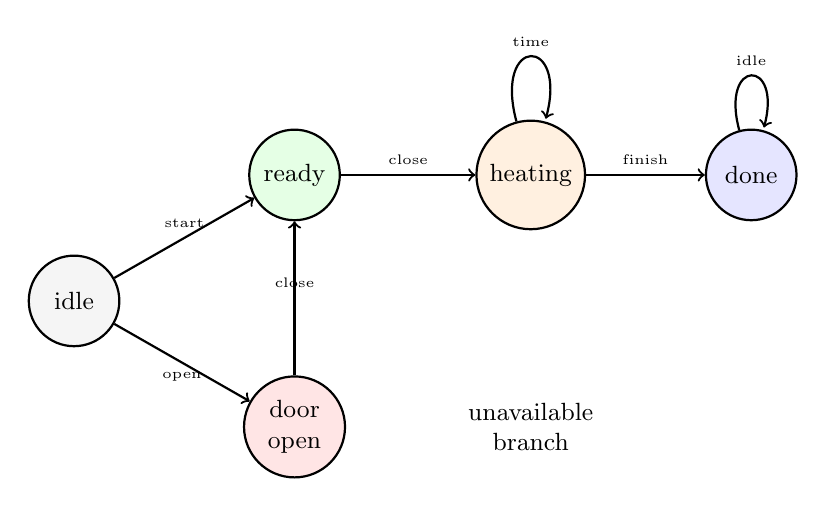
\begin{tikzpicture}[
      st/.style={draw, circle, minimum size=1.15cm, font=\small, thick, align=center},
      arr/.style={->, thick}
    ]
    \node[st, fill=gray!8] (idle) at (0,0) {idle};
    \node[st, fill=green!10] (ready) at (2.8,1.6) {ready};
    \node[st, fill=red!10] (door) at (2.8,-1.6) {door\\open};
    \node[st, fill=orange!12] (heat) at (5.8,1.6) {heating};
    \node[st, fill=blue!10] (done) at (8.6,1.6) {done};
    \node[font=\small, align=center] at (5.8,-1.6) {unavailable\\branch};

    \draw[arr] (idle) -- node[above, font=\tiny] {start} (ready);
    \draw[arr] (idle) -- node[below, font=\tiny] {open} (door);
    \draw[arr] (ready) -- node[above, font=\tiny] {close} (heat);
    \draw[arr] (door) -- node[above, font=\tiny] {close} (ready);
    \draw[arr] (heat) -- node[above, font=\tiny] {finish} (done);
    \draw[arr] (heat) edge[loop above] node[font=\tiny] {time} (heat);
    \draw[arr] (done) edge[loop above] node[font=\tiny] {idle} (done);
  \end{tikzpicture}
  \caption{A branching view of a microwave oven.  From the same state the
           future can split into safe, finishing, or blocked behaviours, and
           CTL can quantify over those branches explicitly.}
  \label{fig:microwave-ctl}
\end{figure}

\subsection{The CTL restriction}

CTL is a fragment of CTL* with a very specific shape.  The restriction is
what makes the logic decidable by the fixed-point algorithms we will use
later.

\begin{definition}[CTL restriction]
A CTL formula is a CTL* formula in which every temporal operator is
immediately preceded by a path quantifier, and path quantifiers do not nest
arbitrarily inside each other.  Informally: temporal structure lives on the
path, but each path must be selected first.
\end{definition}

The restriction is not cosmetic.  It prevents formulas from freely mixing
branching and linear viewpoints inside the same temporal nest.  That trade-off
is exactly what we exploit later: the syntax is narrower than CTL*, but the
resulting model checking problem is much easier to solve.

% =======================================================================
\section{CTL* and Expressiveness}
\label{sec:ctlstar-expressiveness}

CTL* sits above both CTL and LTL.  It is the logic in which state formulas and
path formulas coexist without the CTL restriction.  A CTL* formula may say
``there exists a path where eventually something happens'' just as LTL can,
but it can also say ``on every branch, there is a way to reach a region from
which every continuation satisfies a safety condition'' just as CTL can.

\subsection{Positioning CTL*}

The simplest way to think about CTL* is as the common generalisation of the
two logics already familiar from the book:
\begin{itemize}
  \item LTL is linear-time and talks about one path at a time.
  \item CTL is branching-time and talks about a state by quantifying over
        paths before using temporal operators.
  \item CTL* allows arbitrary nesting of the two styles, so it contains both
        as fragments.
\end{itemize}

\begin{remark}
The price of that extra freedom is not conceptual but algorithmic: CTL* model
checking is still decidable and remains PSPACE-complete, but the formula no
longer has the uniform fixed-point shape that makes CTL particularly pleasant
to evaluate symbolically.
\end{remark}

\subsection{Why CTL and LTL are incomparable}

CTL and LTL are not just different notations for the same class of properties.
Each can express properties the other cannot.

\begin{example}[A CTL property not expressible in LTL]
Consider the branching property
\[
  AG\,EF\,p.
\]
It says that from every reachable state there exists a continuation that can
eventually reach a state satisfying $p$.  The key point is the alternation:
from each state, a fresh existential choice may be made.  LTL cannot express
that kind of branching control because it sees only one path at a time.
\end{example}

\begin{example}[An LTL property not expressible in CTL]
The eventual recurring property
\[
  GF\,p
\]
is linear in spirit: along one execution, $p$ must happen infinitely often.
Its meaning depends on the shape of a single path, not on how many futures
the current state branches into.  CTL cannot isolate that purely linear
behaviour without collapsing the branching structure it is meant to keep.
\end{example}

\medskip\noindent
\textbf{The practical lesson.}  CTL is excellent when specifications are
branching and local, while LTL is excellent when specifications are trace
based.  In engineering work both are used, but they solve different kinds of
questions.

\subsection{The satisfiability boundary}

CTL satisfiability is significantly harder than CTL model checking.

\begin{proposition}[Complexity of CTL satisfiability]
CTL satisfiability is EXPTIME-complete.
\end{proposition}

\medskip\noindent
The point is not only that satisfiability is hard in the worst case.  The
point is that model checking can exploit the finite system model, while
satisfiability must search for any model at all.  Once the model itself is no
longer fixed, the branching possibilities explode much faster.

% =======================================================================
\section{Explicit and Symbolic Model Checking}
\label{sec:symbolic-vs-explicit}

The first model checkers worked explicitly: a state space was built as a graph
and traversed node by node.  That works until the graph becomes too large to
store.  Symbolic model checking changes the representation, not the problem.
States are no longer concrete nodes in memory; they are encoded by Boolean
variables, and sets of states are manipulated as formulas.

\subsection{The state-space explosion}

Suppose a model has $n$ Boolean state variables.  In the worst case there are
$2^n$ concrete states.  Only a tiny fraction may be reachable, but explicit
exploration still has to discover them one by one.  That is the state-space
explosion problem in its cleanest form: the model is compact, the graph is not.

\begin{figure}[ht]
  \centering
  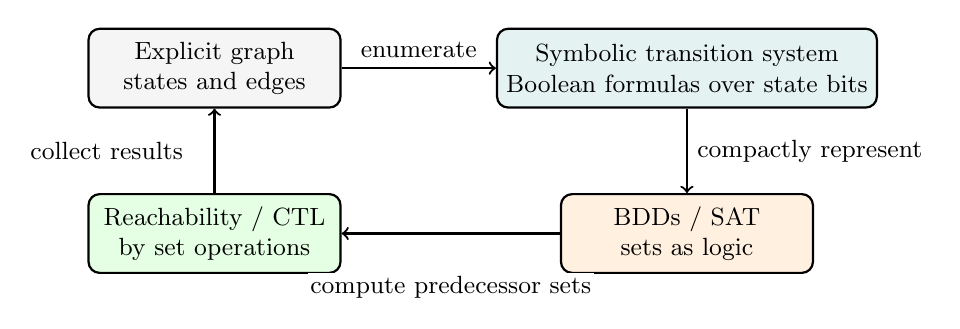
\begin{tikzpicture}[
      box/.style={draw, rounded corners, minimum width=3.2cm,
                  minimum height=1.0cm, align=center, font=\small, thick},
      arr/.style={->, thick}
    ]
    \node[box, fill=gray!8] (explicit) at (0,0) {Explicit graph\\states and edges};
    \node[box, fill=teal!10] (symb) at (6,0) {Symbolic transition system\\Boolean formulas over state bits};
    \node[box, fill=orange!12] (bdd) at (6,-2.1) {BDDs / SAT\\sets as logic};
    \node[box, fill=green!10] (reach) at (0,-2.1) {Reachability / CTL\\by set operations};

    \draw[arr] (explicit) -- node[above, font=\small] {enumerate} (symb);
    \draw[arr] (symb) -- node[right, font=\small] {compactly represent} (bdd);
    \draw[arr] (bdd) -- node[midway, below=14pt, font=\small, fill=white, inner sep=1pt]
      {compute predecessor sets} (reach);
    \draw[arr] (reach) -- node[midway, left=10pt, font=\small, fill=white, inner sep=1pt]
      {collect results} (explicit);
  \end{tikzpicture}
  \caption{Explicit and symbolic model checking solve the same verification
           task, but symbolic methods replace graph storage by Boolean
           representation and Boolean operations.}
  \label{fig:explicit-vs-symbolic}
\end{figure}

\subsection{Symbolic transition systems}

An SMV module is best viewed as a symbolic transition system.  The current
state is not stored as a node in a graph; it is stored as a valuation of
Boolean variables.  If the model uses $n$ Boolean variables, then one concrete
state is just one assignment to
\[
  V = \{x_1,\dots,x_n\}.
\]
The next state uses a primed copy
\[
  V' = \{x_1',\dots,x_n'\},
\]
and the transition relation is a Boolean formula over both sets of variables.
That is the bridge from an explicit Kripke structure to the SMV style of
representation.

\begin{definition}[Symbolic transition system]
Let $V = \{x_1,\dots,x_n\}$ be a finite set of Boolean variables and let
$V' = \{x_1',\dots,x_n'\}$ be their next-state copies.  A symbolic transition
system consists of three Boolean formulas:
\begin{itemize}
  \item $Init(V)$, describing the initial states;
  \item $T(V,V')$, describing the transition relation;
  \item $L_p(V)$ for each atomic proposition $p$, describing where $p$ holds.
\end{itemize}
\end{definition}

To see the conversion explicitly, take a finite Kripke structure
$\mathcal{M} = (Q, I, R, L)$.  Choose enough Boolean variables to encode every
state in $Q$, and fix an encoding function
\[
  enc : Q \to \{0,1\}^n.
\]
Then the three symbolic formulas are obtained by collecting the encodings of
the corresponding explicit sets:
\[
  Init(V) = \bigvee_{q \in I} enc(q),
  \qquad
  T(V,V') = \bigvee_{(q,q') \in R} enc(q) \land enc'(q'),
\]
\[
  L_p(V) = \bigvee_{q \in L(p)} enc(q).
\]
Here $enc'(q')$ is the same bit pattern as $enc(q')$, but written on the
primed variables.  In other words, an initial set becomes a disjunction of
encoded states, a transition becomes a disjunction of encoded state pairs, and
each atomic proposition becomes the disjunction of all states where that label
is true.

\begin{example}[A concrete SMV-style encoding]
Suppose the explicit model is a 2-bit modulo-4 counter with bits
$b_1,b_0$.  The initial state is $00$, so
\[
  Init(b_1,b_0) = \neg b_1 \land \neg b_0.
\]
The transition relation says that the counter increments by one modulo $4$:
\[
  T(b_1,b_0,b_1',b_0') =
    (b_0' \leftrightarrow \neg b_0)
    \land
    (b_1' \leftrightarrow (b_1 \oplus b_0)).
\]
If $p$ means ``the counter is at state $3$'', then
\[
  L_p(b_1,b_0) = b_1 \land b_0.
\]
The explicit graph has four nodes and four edges, but the symbolic
representation stores the whole model with one initial formula, one transition
formula, and one label formula.
\end{example}

\begin{figure}[ht]
  \centering
  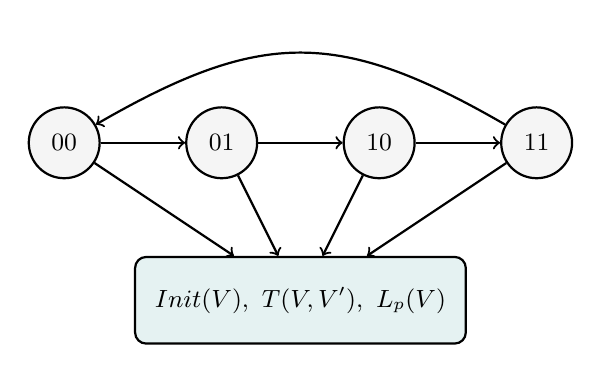
\begin{tikzpicture}[
      st/.style={draw, circle, minimum size=9mm, font=\small, thick},
      box/.style={draw, rounded corners, minimum width=4.2cm,
                  minimum height=1.1cm, align=center, font=\small, thick},
      arr/.style={->, thick}
    ]
    \node[st, fill=gray!8] (s0) at (0,0) {$00$};
    \node[st, fill=gray!8] (s1) at (2.0,0) {$01$};
    \node[st, fill=gray!8] (s2) at (4.0,0) {$10$};
    \node[st, fill=gray!8] (s3) at (6.0,0) {$11$};
    \node[box, fill=teal!10] (symb) at (3.0,-2.0)
      {$Init(V),\ T(V,V'),\ L_p(V)$};

    \draw[arr] (s0) -- (s1);
    \draw[arr] (s1) -- (s2);
    \draw[arr] (s2) -- (s3);
    \draw[arr] (s3) to[out=150,in=30,looseness=1.2] (s0);

    \draw[arr] (s1) -- (symb);
    \draw[arr] (s2) -- (symb);
    \draw[arr] (s3) -- (symb);
    \draw[arr] (s0) -- (symb);
  \end{tikzpicture}
  \caption{A finite explicit model is encoded by Boolean variables, then
           collapsed into an initial condition, a transition formula, and
           label formulas over those variables.}
  \label{fig:smv-bridge}
\end{figure}

The SMV syntax from Chapter~\ref{ch:reactive-smv} is simply a structured way
to write those formulas.  A variable declaration becomes part of the state
encoding; an assignment to \texttt{next} becomes a conjunct of $T$; a
specification becomes a property over the reachable set.

\medskip\noindent
\textbf{Why this is powerful.}  A symbolic transition system can have an
enormous implicit graph while still using only a short formula to describe it.
If $n$ Boolean variables are enough to encode the model, then the explicit
state graph may have up to $2^n$ states and $2^n \cdot 2^n$ possible pairs of
states, but the symbolic description still has size polynomial in $n$ and in
the structure of the formulas.  This is the source of the exponential
succinctness: the representation size grows with the number of bits, while the
set of represented states grows with the number of valuations.

That is the main reason symbolic checking scales better than explicit
enumeration on many real hardware models.

\subsection{Symbolic reachability}

Reachability is the core operation behind symbolic model checking.  Instead of
following one edge at a time, we compute sets of successors and predecessors.
For a set of states $Z$, the existential predecessor operator is
\[
  Pre_E(Z) = \{\, s \mid \exists s'.\ T(s,s') \land s' \in Z \,\}.
\]
Its universal dual is
\[
  Pre_A(Z) = \{\, s \mid \forall s'.\ T(s,s') \rightarrow s' \in Z \,\}.
\]
With these two operators, the symbolic view of model checking becomes a game
of set iteration.

\begin{example}[A symbolic intuition]
Suppose we want to know which states can reach a safe shutdown state.  In an
explicit graph we would mark predecessors one edge at a time.  In the symbolic
view we keep a Boolean formula for the current set, compute its predecessor by
one formula transformation, and repeat until the set stops growing.
\end{example}

% =======================================================================
\section{Bounded Model Checking and OBDDs}
\label{sec:bmc-obdd}

\subsection{Bounded model checking}

Symbolic checking is still exhaustive.  Bounded model checking is not, at
least not by itself.  It is a different use of the same symbolic machinery:
instead of computing a whole fixed point, we ask whether there exists a short
counterexample of length at most $k$.

\begin{definition}[Bounded model checking]
Given a transition system $\mathcal{M}$ and a property $\varphi$, bounded
model checking asks whether there exists a path of length at most $k$ from an
initial state of $\mathcal{M}$ that violates $\varphi$.  The question is
encoded as a propositional satisfiability problem.
\end{definition}

The unrolling is direct, but it helps to see one concrete instance all the way
through.  Consider a tiny two-bit transition system with state variables
$x_1,x_0$.  The initial state is
\[
  Init(x_1,x_0) \equiv \neg x_1 \land \neg x_0,
\]
so the machine starts in state $00$.  Its next-state relation is the binary
incrementer modulo four:
\[
  x_0' \leftrightarrow \neg x_0, \qquad
  x_1' \leftrightarrow (x_1 \oplus x_0).
\]
Starting from $00$, the unique execution is $00 \to 01 \to 10 \to 11 \to 00$.
Suppose that $11$ is the bad state, and we want a counterexample to the safety
property $AG\,\neg \texttt{bad}$.

For a bound $k=3$, we create four copies of the state variables:
\[
  (x_1^0,x_0^0),\ (x_1^1,x_0^1),\ (x_1^2,x_0^2),\ (x_1^3,x_0^3).
\]
The SAT instance is then built in three steps:
\begin{enumerate}
  \item \textbf{Initial state.}  Fix the first copy to satisfy the initial
        condition:
        \[
          Init(x_1^0,x_0^0).
        \]
  \item \textbf{Transition relation.}  Constrain every adjacent pair of
        copies to follow the transition relation:
        \[
          \bigwedge_{i=0}^{2}
          \Bigl((x_0^{i+1} \leftrightarrow \neg x_0^i) \land
                (x_1^{i+1} \leftrightarrow (x_1^i \oplus x_0^i))\Bigr).
        \]
  \item \textbf{Bad prefix.}  Ask that the bad state is reached at some point
        within the bound:
        \[
          Bad_3 \equiv
          (x_1^0 \land x_0^0) \lor
          (x_1^1 \land x_0^1) \lor
          (x_1^2 \land x_0^2) \lor
          (x_1^3 \land x_0^3).
        \]
\end{enumerate}
Putting the pieces together, the bounded counterexample formula is
\[
  \Phi_3 =
  Init(x_1^0,x_0^0)
  \land \bigwedge_{i=0}^{2}
    \Bigl((x_0^{i+1} \leftrightarrow \neg x_0^i) \land
          (x_1^{i+1} \leftrightarrow (x_1^i \oplus x_0^i))\Bigr)
  \land Bad_3.
\]
This formula is satisfiable, with the witness trace
\[
  00,\ 01,\ 10,\ 11,
\]
which is exactly the counterexample we expected.

That is the general pattern.  The state variables are replicated for each time
frame, the initial condition anchors the first frame, the transition relation
connects consecutive frames, and the negation of the property is asserted on
the unrolled prefix.  For safety properties this often means ``some bad state
appears within $k$ steps''; for richer formulas, the bad condition is encoded
by translating the temporal operators over the bounded prefix.

\medskip\noindent
\textbf{What BMC buys.}  SAT solvers are very good at proving the existence of
short bad behaviours.  That is why BMC is often used as a bug-finding mode:
fast for shallow errors, incomplete unless a completeness threshold is
reached.

\subsection{From binary decision trees to OBDDs}

The other symbolic workhorse is the ordered binary decision diagram, usually
called an OBDD.  It is a compressed representation of a Boolean function.

\begin{definition}[OBDD]
An \emph{ordered binary decision diagram} is a reduced binary decision graph
in which every internal node is labelled by a Boolean variable, variables
appear in the same fixed order along every path, and repeated subgraphs are
shared.
\end{definition}

The starting point is a binary decision tree.  Every internal node asks one
variable, every edge corresponds to the value $0$ or $1$, and every leaf is a
Boolean constant.  The OBDD is what remains after we remove redundant tests
and merge identical subtrees.

At the algebraic level this is just Shannon expansion:
\[
  f = (\neg x \land f|_{x=0}) \lor (x \land f|_{x=1}).
\]
An OBDD is the DAG form of that expansion, with one fixed variable order
shared by every path.

\begin{figure}[ht]
  \centering
  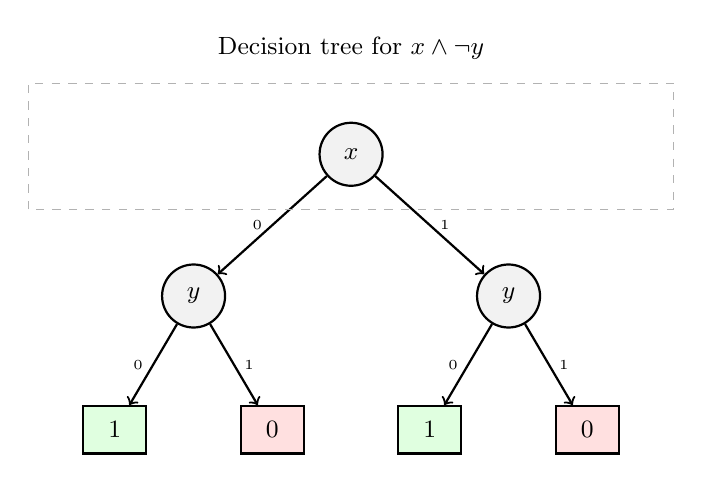
\begin{tikzpicture}[
      node/.style={circle, draw, thick, minimum size=8mm, font=\small},
      leaf/.style={rectangle, draw, thick, minimum width=8mm, minimum height=6mm, font=\small},
      arr/.style={->, thick}
    ]
    \node[node, fill=gray!10] (x) at (0,0) {$x$};
    \node[node, fill=gray!10] (y1) at (-2,-1.8) {$y$};
    \node[node, fill=gray!10] (y2) at (2,-1.8) {$y$};
    \node[leaf, fill=green!12] (t1) at (-3,-3.5) {$1$};
    \node[leaf, fill=red!12] (f1) at (-1,-3.5) {$0$};
    \node[leaf, fill=green!12] (t2) at (1,-3.5) {$1$};
    \node[leaf, fill=red!12] (f2) at (3,-3.5) {$0$};
    \draw[arr] (x) -- node[left, font=\tiny] {$0$} (y1);
    \draw[arr] (x) -- node[right, font=\tiny] {$1$} (y2);
    \draw[arr] (y1) -- node[left, font=\tiny] {$0$} (t1);
    \draw[arr] (y1) -- node[right, font=\tiny] {$1$} (f1);
    \draw[arr] (y2) -- node[left, font=\tiny] {$0$} (t2);
    \draw[arr] (y2) -- node[right, font=\tiny] {$1$} (f2);
    \draw[dashed, gray!60] (-4.1,-0.7) rectangle (4.1,0.9);
    \node[font=\small] at (0,1.35) {Decision tree for $x \wedge \neg y$};
  \end{tikzpicture}
  \caption{A small decision tree.  The OBDD is obtained by fixing an order,
           removing duplicated tests, and merging equal subtrees.  For this
           example, the reduced form is already close to the tree.}
  \label{fig:decision-tree-obdd}
\end{figure}

\begin{example}[Ordering-sensitive equality]
Let
\[
  eq(x_1,x_0,y_1,y_0) \equiv
  (x_1 \leftrightarrow y_1) \land (x_0 \leftrightarrow y_0).
\]
With the order $x_1,y_1,x_0,y_0$, the diagram can reject a mismatch in the
high bits immediately and only needs to remember whether the first pair
agreed.  The same idea works for the low bits, so the graph stays small.

With the order $x_1,x_0,y_1,y_0$, the diagram must first distinguish all four
possibilities for $x_1x_0$ before it has even seen the $y$ bits.  Those four
partial cases lead to different residual functions, so the OBDD grows much
larger.  The Boolean function is unchanged; only the order changed.
\end{example}

\subsection{The restrict function}

The recursive algorithms for OBDDs are built around variable restriction.
For a Boolean function $f$ and a variable $x$,
\[
  f|_{x=0} \quad\text{and}\quad f|_{x=1}
\]
are the cofactors of $f$ obtained by fixing $x$.

\begin{definition}[Restrict]
\label{def:restrict}
The restrict operation returns the function obtained by assigning a Boolean
value to one variable and simplifying the result.
\end{definition}

The meaning is easiest to see on a formula such as
\[
  f(x,y,z) = (x \land y) \lor z.
\]
Then
\[
  f|_{x=0} = z
  \qquad\text{and}\qquad
  f|_{x=1} = y \lor z.
\]
The point of restriction is that it turns one Boolean function into the two
smaller functions that appear in its Shannon expansion.  With that operation,
an OBDD can be built recursively: pick the first variable in the global
order, compute the two cofactors, build the two sub-OBDDs, and merge them if
they are identical.  The same idea underlies the standard Boolean operations
on OBDDs: to compute $f \mathbin{\circ} g$, recursively combine the cofactors
of the two inputs and memoise the intermediate results.

\medskip\noindent
\textbf{Negation is the easiest case.}  If an OBDD already represents $f$, the
graph for $\neg f$ has the same internal tests and the same sharing pattern;
only the terminal values change.  Intuitively, every path that used to end in
$0$ now ends in $1$, and vice versa.  In a reduced OBDD this is why
complementation is so cheap: the variable order and the structure do not need
to be rebuilt from scratch.

\subsection{Why ordering matters}

\begin{example}[Ordering sensitivity]
Two equivalent Boolean functions may have OBDDs of wildly different sizes
under different variable orders.  The reason is structural: an OBDD is not a
free graph but a graph constrained by the order.  A good order exposes shared
subfunctions; a bad order hides them.
\end{example}

This sensitivity is the main practical caveat of OBDDs.  In return, when the
order is good, Boolean operations become efficient and the representation can
be dramatically smaller than the full truth table.  That is why BDD packages
remain central to symbolic verification tools.

% =======================================================================
\section{CTL by Predicate Transformers and Fixed Points}
\label{sec:ctl-fixed-points}

The deepest algorithmic view of CTL is not graph-theoretic but algebraic.
Instead of asking ``which path satisfies this formula?'' we ask ``which set of
states satisfies it?''  That set is obtained by applying monotone predicate
transformers until a fixed point is reached.

This viewpoint is useful because it matches the shape of the properties
themselves.  Reachability grows outward from a base case: first we know where
the goal already holds, then we add states that can step into that set.  That
is exactly the behaviour of a least fixed point.  Invariance works in the
opposite direction: we begin with all states and remove the ones that can
escape the safe region, so the approximation shrinks toward a greatest fixed
point.

\subsection{Predecessor transformers}

The two basic symbolic transformers were already introduced in the reachability
section:
\[
  Pre_E(Z) = \{\, s \mid \exists s'.\ T(s,s') \land s' \in Z \,\}
\]
\[
  Pre_A(Z) = \{\, s \mid \forall s'.\ T(s,s') \rightarrow s' \in Z \,\}
\]
They are the existential and universal predecessor operators.  The first asks
whether there is at least one successor in $Z$; the second asks whether all
successors stay in $Z$.

\begin{note}
In symbolic implementations these operators are formula transformations.  With
state formulas encoded as Boolean formulas, $Pre_E$ is typically computed by
existentially quantifying next-state variables, while $Pre_A$ is derived by
duality.
\end{note}

\subsection{Fixed-point characterisations}

CTL model checking becomes a matter of computing least and greatest fixed
points over sets of states.

\begin{proposition}[CTL as fixed points]
Let $\llbracket \varphi \rrbracket$ denote the set of states satisfying the
CTL formula $\varphi$.  Then:
\[
  \llbracket EF\,\varphi \rrbracket = \mu Z.\ \llbracket \varphi \rrbracket \cup Pre_E(Z)
\]
\[
  \llbracket EG\,\varphi \rrbracket = \nu Z.\ \llbracket \varphi \rrbracket \cap Pre_E(Z)
\]
\[
  \llbracket AF\,\varphi \rrbracket = \mu Z.\ \llbracket \varphi \rrbracket \cup Pre_A(Z)
\]
\[
  \llbracket AG\,\varphi \rrbracket = \nu Z.\ \llbracket \varphi \rrbracket \cap Pre_A(Z)
\]
\[
  \llbracket E[\varphi_1 U \varphi_2] \rrbracket
  = \mu Z.\ \llbracket \varphi_2 \rrbracket \cup
    \bigl(\llbracket \varphi_1 \rrbracket \cap Pre_E(Z)\bigr)
\]
\[
  \llbracket A[\varphi_1 U \varphi_2] \rrbracket
  = \mu Z.\ \llbracket \varphi_2 \rrbracket \cup
    \bigl(\llbracket \varphi_1 \rrbracket \cap Pre_A(Z)\bigr)
\]
\end{proposition}

The meaning of the notation is straightforward, but the algorithmic intuition
is worth spelling out.  A least fixed point $\mu Z.\,F(Z)$ is the smallest set
that is closed under the rule encoded by $F$.  We discover it by starting from
the empty set and repeatedly adding states that are justified by the rule.
That is why least fixed points describe reachability: a state belongs to the
result only if there is a finite chain of justifications that leads back to
the base case.

A greatest fixed point $\nu Z.\,F(Z)$ is the largest set that survives the
rule.  We discover it by starting from the whole state space and repeatedly
removing states that cannot justify themselves.  That is why greatest fixed
points describe invariance or ``always'' properties: a state belongs to the
result only if every step can stay inside the candidate set forever.

\subsection{The iteration view}

These equations turn into simple loops.  The loop variable is not just a
technical artefact: it is the current approximation to the answer.
\begin{itemize}
  \item For a least fixed point, initialise $Z_0 = \emptyset$ and repeatedly
        set $Z_{i+1} = F(Z_i)$.  At each pass, $Z_i$ contains the states whose
        correctness has already been justified by a path of length at most
        $i$.
  \item For a greatest fixed point, initialise $Z_0$ to all states and
        repeatedly set $Z_{i+1} = F(Z_i)$.  At each pass, $Z_i$ contains the
        states that have not yet been disproved as safe or persistent.
\end{itemize}

\begin{formaldetails}[Why the iteration is correct]
The critical fact is monotonicity: if $Z \subseteq Z'$, then $F(Z) \subseteq
F(Z')$.  That single property gives the loop its invariant.

For a least fixed point, every iterate is an under-approximation:
$Z_0 \subseteq Z_1 \subseteq \cdots$, and each new set only adds states whose
membership is already supported by the previous approximation.  Nothing enters
the set ``too early'', because a state can only be added when one of its
predecessors is already known to be good, or the base case already holds.

For a greatest fixed point, every iterate is an over-approximation:
$Z_0 \supseteq Z_1 \supseteq \cdots$, and each new set only removes states
that fail the preservation check.  Nothing is removed ``too soon'', because a
state stays in the candidate set exactly when all of its successors still lie
inside the current approximation.

Since the state space is finite, the chain cannot keep changing forever.  The
least-fixed-point loop eventually reaches the first set that is closed under
the rule, and the greatest-fixed-point loop eventually reaches the largest set
that survives it.  At that moment the current approximation is a fixed point,
and the loop invariant tells us it is the least or greatest one we wanted.
\end{formaldetails}

\medskip\noindent
\textbf{How this reads operationally.}  A CTL checker does not ``search the
tree'' in the naive sense.  It repeatedly computes preimages of sets until the
sets stop changing.  The current set is the worklist of states already proved
good, and the predecessor transformer is the step that tries to extend that
proof by one transition.  That is the algebraic core of the standard CTL
algorithm.

\subsection{A worked reading of the formulas}

The fixed-point view explains the usual CTL operators very cleanly:
\begin{itemize}
  \item $EF\,\varphi$ is the set of states from which $\varphi$ is reachable
        along some path.
  \item $AF\,\varphi$ is the set of states from which every path is
        eventually forced into $\varphi$.
  \item $EG\,\varphi$ is the set of states that can stay inside $\varphi$
        forever by following some branch.
  \item $AG\,\varphi$ is the set of states from which no branch can escape
        $\varphi$.
\end{itemize}

\subsection{Worked derivation: $AF$ as a least fixed point}

The operator $AF\,\varphi$ is the cleanest place to see the algorithm at
work.  Intuitively, a state satisfies $AF\,\varphi$ when every path from that
state is forced to encounter a $\varphi$-state eventually.  The fixed-point
equation
\[
  \llbracket AF\,\varphi \rrbracket = \mu Z.\ \llbracket \varphi \rrbracket \cup Pre_A(Z)
\]
says exactly that a state is good for one of two reasons: either $\varphi$ is
already true there, or every successor is already known to be good.

Write $F(Z) = \llbracket \varphi \rrbracket \cup Pre_A(Z)$.  Then the
iteration is:
\[
  Z_0 = \emptyset,\qquad Z_{i+1} = F(Z_i).
\]
Now read the first few rounds as a proof search.
\begin{itemize}
  \item $Z_1 = \llbracket \varphi \rrbracket$.  In one step we discover the
        states where the goal is already true.
  \item $Z_2$ adds every state whose successors are all in $Z_1$.  These are
        states from which $\varphi$ is guaranteed within one transition.
  \item $Z_3$ adds states whose successors are all in $Z_2$.  These are the
        states that are guaranteed to reach $\varphi$ within two transitions.
  \item And so on.  At stage $i$, $Z_i$ contains precisely the states from
        which $\varphi$ is forced within at most $i-1$ steps.
\end{itemize}

The limit of that chain is the set of states from which no path can avoid
eventually hitting $\varphi$.  If a state were missing from the limit, then
there would be a branch that keeps escaping the candidate set forever, and the
universal predecessor test would never be able to certify it.  If a state is
in the limit, then some finite round has already established the bound on when
$\varphi$ must appear.

The same style of argument works for $EG\,\varphi$, but with the quantifiers
reversed.  There the loop starts from all states, keeps only those that have a
successor still inside the candidate set, and converges to the largest region
from which one can stay in $\varphi$ forever.  So the fixed point is not just
an abstract denotation: it is the exact form of the algorithm.

% =======================================================================
\section{Summary}
\label{sec:ctl-summary}

\begin{summarybox}
\begin{itemize}[nosep]
  \item CTL is a branching-time logic: each temporal operator is preceded by
        either an existential or a universal path quantifier.
  \item CTL* is the larger logic that contains both CTL and LTL.  CTL and
        LTL are incomparable in expressive power.
  \item CTL satisfiability is EXPTIME-complete, while model checking becomes
        efficient because the model is fixed and finite.
  \item Symbolic model checking replaces explicit graph traversal by Boolean
        formulas over state variables, transition relations, and predecessor
        set computations.
  \item Bounded model checking searches for short counterexamples by turning
        a bounded unrolling into a SAT instance.
  \item OBDDs compactly represent Boolean functions once a variable order is
        fixed, but the size can depend strongly on that order.
  \item CTL model checking can be written as a collection of least and
        greatest fixed points over predecessor transformers.
\end{itemize}
\end{summarybox}
